\subsection{Precision sensitivity on the OpenAI datasets}
\label{sec:7-precision}

Supplementary source inspection establishes that the E1 implementation
uses TF32 multiplication with FP32 accumulation for OpenAI rotation and
centroid GEMMs, despite FP32 input/storage and a misleading source comment
(\cref{sec:4-2}). The main E1 frontier remains the historical measurement
of that implementation. A separate FP32 variant changes the cuBLAS
math-mode switch and replays 37/39 OpenAI configurations at batch 1,000,
five rounds each. Execution order alternates between variants across
probe settings. Both reuse the same TF32-trained model; the intervention
changes add/query arithmetic, including database encoding and routing.
It is not a comparison of independently FP32-trained models.
\Cref{tab:7-precision} summarises the paired changes.

\par\medskip\noindent\begin{minipage}{\linewidth}
\centering\captionsetup{hypcap=false}
\captionof{table}[FP32 sensitivity at matched configurations]{FP32 sensitivity. QPS ratio is FP32/TF32 at equal configuration
(geometric mean); recall differences have the same direction. The last
two columns compare the FP32 frontier at recall 0.97 with archived E1
IVF-RaBitQ and CAGRA fp32 frontiers. Baselines were not remeasured.}
\label{tab:7-precision}
\scriptsize\setlength{\tabcolsep}{3pt}
\begin{tabular}{@{}lrrrrr@{}}
\toprule
Dataset & Pairs & QPS ratio & $\Delta$Recall & vs RaBitQ & vs CAGRA \\
\midrule
OpenAI-1536 & 37 & 0.953 & +0.0003--+0.0005 & 1.086 & 1.679 \\
OpenAI-3072 & 39 & 0.951 & +0.0000--+0.0003 & 1.079 & 1.629 \\
\bottomrule
\end{tabular}

\end{minipage}\par\medskip

At equal configuration, FP32 reduces throughput by about 5\% and increases
recall by 0--0.0005. At matched recall 0.97, its throughput is about 3\%
below the same-session TF32 frontier. It remains $1.086\times$ and
$1.079\times$ archived RaBitQ, and $1.679\times$ and $1.629\times$
archived CAGRA fp32. Same-session v69/RaBitQ ratios are 1.118/1.114,
versus historical 1.130/1.157. This separates the precision intervention
from session variation: the competitive direction persists, with smaller
margins, while the cross-session baseline comparison retains timing
uncertainty. The two precision variants' complete frontiers are shown in
\cref{fig:7-precision}.

\begin{figure}[tbp]
\centering
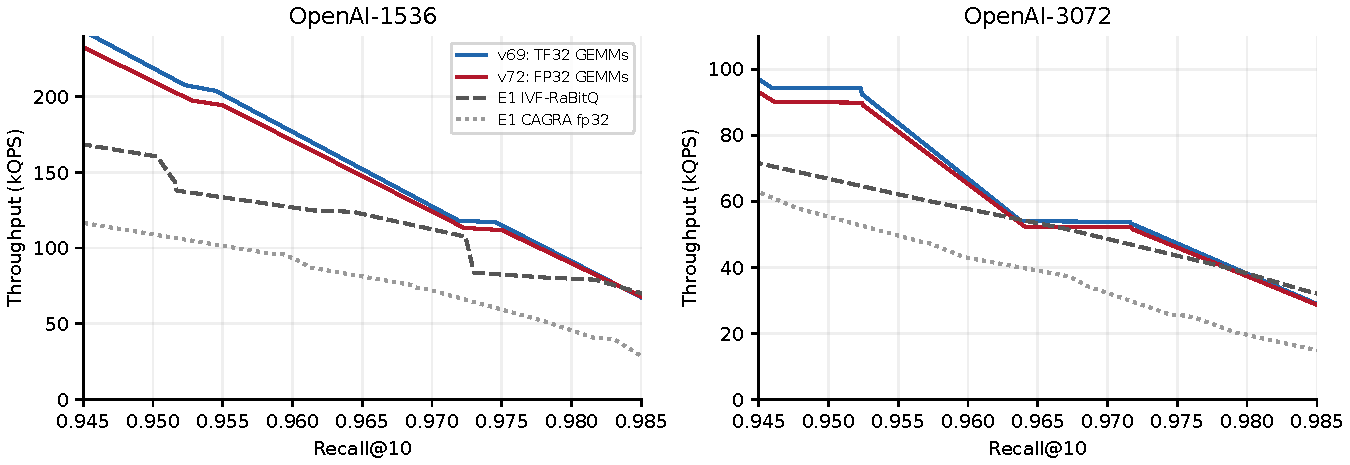
\includegraphics[width=\linewidth]{supplement/precision.pdf}
\caption[TF32 and FP32 precision frontiers]{Supplementary precision frontiers. Solid curves are same-session
JHQ variants; dashed/dotted baselines are historical E1 measurements.
All use the chapter's frontier and interpolation rules.}
\label{fig:7-precision}
\end{figure}
